\ifdefined\included
\else
\setcounter{chapter}{2} %% Numéro du chapitre précédent ;)
\dominitoc
\faketableofcontents
\fi

\chapter{HATEB-2 for Legible Proactive Planning with Situation Analysis}
\minitoc
\chaptermark{Proactive Planning with Situation Analysis}
\label{chap:3}
\section{Introduction}

%%%%%%% Could be a part of chapter 2 or Intro %%%%%%%%%
% The study of human-aware navigation, sometimes, called social navigation is increasing day by day as assistive robots are being deployed at various places like airports, malls \cite{10.1007/978-3-319-47437-3_74}, hospitals etc. Various methods of human-aware navigation are proposed, and most of them are based on the theory of proxemics \cite{hall_book_1966} and social force model \cite{helbing1995social}. Many of the earlier proposed methods, however, do not use human predictions in the planning and hence faced difficulties in complex situations. Consequently, human motion predictions and estimations were introduced into human-aware navigation to have a better planning system. 
%%%%%%%%%%%%%%%%%%%%%%%%%%%%%%%%%%%%%%%%%%%%%%%%%%%%%%%

% In Human Aware Timed Elastic Band (HATEB) based co-navigation planner \cite{khambhaita2017viewing} falls into this category, including human estimations and predictions. 

\acrfull{hateb}~\cite{khambhaita2017viewing} includes human predictions by simultaneously planning for humans and the robot. This allows \acrshort{hateb} to handle intricate situations like narrow corridor crossing and door crossing, where human and robot cooperative motion is needed. With the increasing complexity of environments and the need to navigate robots in such environments, decision-making has been introduced into planning~\cite{qian2013decision, mehta2016autonomous}. However, these frameworks might make the robot wait in confined spaces instead of proactively planning, hence, resulting in larger execution times. Therefore, in this chapter, we propose HATEB-2, a new modality based human-robot co-navigation framework that uses decision-making to solve semi-crowded as well as intricate scenarios. This is achieved by shifting between different modalities and simultaneous human-robot planning, similar to \acrshort{hateb}. This chapter discusses the following three things in detail: 1) HATEB-2, a new human-robot co-navigation planner comprising decision-making. 2) Improvements and modifications to \acrshort{hateb}. 3) Analysis of human-robot co-navigation in a variety of situations. 

Note that this chapter discusses only the first version of HATEB-2 and its implementation. The subsequent chapters of this thesis discuss the evolution of this planner over time. Throughout this chapter, humans are represented as green cylinders with yellow arrows, where the direction of the arrows corresponds to the frontal direction of humans. 

The chapter is organised as follows. Section~\ref{chap3_related_work} presents the related work corresponding to this chapter. Section \ref{proactive_planning} briefly presents the proactive planning in \acrshort{hateb} and the \textit{`entanglement problem'}. Section~\ref{SA_mode} presents the architecture of HATEB-2, describes the different modes of planning and finally explains the modality shifting process based on the situation assessment. Following this, section~\ref{improve_legible} presents the modifications to \acrshort{hateb} and the new human-aware constraints. The results and the analyses of the proposed architecture in various simulated experiments are presented in section~\ref{results_chap3}, and the tests in the real world are presented in section~\ref{real_chap3}. Section~\ref{conclude_chap3} finally concludes this chapter.

\section{Related Work}\label{chap3_related_work}
Most state-of-art \acrshort{han} planners use proxemics zones around humans in a grid-based map representation of the robot's working environment~\cite{kruse_ras_2013}. Nonetheless, proxemics alone may not be sufficient to generate completely human-acceptable motion for the robot. Sometimes planning approaches like \acrshort{sfm}~\cite{helbing1995social, ferrer2013robot} and velocity-obstacle models~\cite{snape2011hybrid, berg2011reciprocal} are also used for HAN. As these approaches are reactive, they do not necessarily produce legible robot motion. In the human-aware navigation planner proposed by Sisbot et al.~\cite{sisbot_tr_2007}, other social criteria like visibility and hidden zones were considered along with the proxemics. Another framework proposed by Kruse et al.~\cite{kruse_arso_2012} introduced the directional cost model, which attempts to solve the spatial conflict by adjusting velocity instead of the path whenever possible. The study conducted by Kruse et al.~\cite{kruse2014evaluating} showed that humans prefer the robot to follow this strategy, especially in path crossing scenarios. This model has also been shown to increase the legibility of the robot motions, and hence, in HATEB-2, we introduced some new constraints that restrict the path change and adjust the velocity based on the distance between the human and the robot. 

Employing social constraints alone may not be sufficient to develop a socially acceptable navigation planner, and this raises the need for including human motion predictions into the framework~\cite{kuderer_rss_2012}. Many methods based on the \acrshort{sfm} predict homotopically distinct trajectories for humans and design planners that learn the navigation policies for the robot based on human demonstrations~\cite{kuderer_rss_2012}. Although these methods involving independent human predictions work fine in large open spaces, they might require to re-learn the parameters to handle situations such as passing through a long corridor or a door, where coordination is needed between humans and the robot. Hence planning for humans along with the robot is required in such situations. The approach presented by Ferrer et al.~\cite{ferrer2015multi} uses the \acrshort{sfm}, both for predicting human paths and controlling the robot's motion. In this approach, human predictions based on the previously planned paths were used. Other approaches~\cite{bordallo_iros_2015, nagariya_cdc_2015} try to predict the possible human goals based on some type of reasoning and generate locally optimal motion for the robot. One of the recent approaches~\cite{fisac2018probabilistically} suggests the use of probabilistic human predictions to handle various uncertainties and plan the robot's motion on top of these probabilistic predictions. This approach is particularly useful in systems with unreliable sensors. All these approaches are effective in densely crowded environments as a virtue of remaining purely reactive but can lead to needless detours in intricate situations. Our previous work~\cite{khambhaita2017viewing} is specifically developed to handle such intricate situations in semi-crowded environments. Such planning for humans along with the robot is usually required in robot-human handover scenarios to know where to perform a task and who performs a task~\cite{mainprice_ro-man_2012,waldhart_iros_2015}. 

The concept of modality shifting in human-aware navigation is discussed in works by Mehta et al.~\cite{mehta2016autonomous} and Qian et al.~\cite{qian2013decision}, where \acrshort{pomdp} is used for decision making. In both works, different modalities necessary for human-aware navigation are proposed, assuming that the robot takes all the load of the navigation process. Hence these methods may also suffer problems like purely reactive planners in complex situations leading to unnecessary detours or long halts. HATEB-2 includes \acrshort{hateb} as one of the modalities and hence can handle both intricate as well as semi-crowded scenarios by switching between different modalities when needed. In this chapter, however, we focus mainly on different intricate situations involving cooperative motion between the human and the robot. 

% \textcolor{red}{add related works for proactive planning and situation assessment}

\section{Proactive Planning in HATEB}
\label{proactive_planning}
As presented in Chapter \ref{chap:1}, the formulation of \acrshort{hateb} allows us to plan for the robot and the humans involved in the interaction simultaneously. As this approach plans for all the agents, the robot's trajectory can be proactively updated before something happens. Hence, it can solve human-robot navigation scenarios in a better way when compared to reactive-only schemes. However, some assumptions made about humans during this formulation and the structure of its implementation can lead to deadlock situations, as shown in Fig. \ref{stuck}. We call it the `\textit{entanglement problem}' throughout this thesis, and its details are presented below.

\subsection{The Entanglement Problem}
In \acrshort{hateb}, the robot's trajectory is adapted based on the predicted humans' (planned) trajectories. While planning, it considers a constant velocity for humans and assumes that they are always in motion. Hence, if the human stops moving, the system keeps anticipating the human movement in the immediate time step. One more issue is that the path prediction system for humans is called only once at the start of the planning, and it puts more burden on trajectory planning to handle the discrepancies. The assumptions about the agents and this planning strategy result in the `\textit{entanglement}' of trajectories when the human stops moving, and the robot is stuck, waiting for the human to move. These situations can occur commonly in corridors, and two such situations are shown in Fig.  \ref{stuck}. The optimization scheme neglects the other possible solutions as these trajectories have the minimum cost. This leads to another case of the \acrfull{frp} even when there is enough space to move. We address this issue in HATEB-2 by detecting such situations and then taking mitigating actions.

\begin{figure}[!h]
\centering
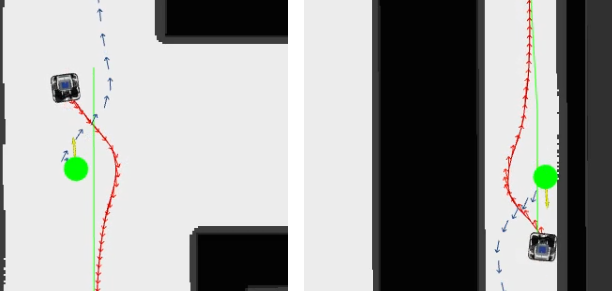
\includegraphics[width=0.9\columnwidth]{images/chapter3/entanglement_cut.png}
\caption{Robot getting stuck due to \textit{entanglement} of trajectories. The poses in blue correspond to the human's trajectory and the ones in red to the robot's trajectory. In the situations shown, there exists an alternate solution for the robot to solve the problem. However, the assumption about the human having non-zero velocity and the safety constraint makes the robot wait in the same entanglement, speculating the motion of the human. The picture on the left is of open space, whereas the one on the right is of a narrow corridor.}
\label{stuck}
\end{figure}

\section{HATEB-2: Situation Analysis and Mode Shifting}\label{SA_mode}
The proposed framework, HATEB-2, combines decision-making and planning into a single framework and opens up new frontiers for HAN planning. This new framework can encompass a large variety of problems by allowing the transition between different modalities based on context. In this chapter, however, we study only the human-robot co-navigation problem. HATEB-2 introduces decision-making on top of planning, and this makes the planner adapt better to the situations at hand. These situations might be very different from each other and need to be handled differently. A single way of planning may not be sufficient in such situations, and hence, we introduce three different modalities into planning. All these modalities use \acrfull{teb}~\cite{rosmann2013efficient} as their base, and the transition between them is handled by the decision-making loop.

% TEB is one of the well-known approaches for robot navigation around dynamic obstacles, which allows us to include several kinodynamic and custom constraints  (like holonomic, non-holonomic, human-aware constraints) into the local reactive planning. TEB is modelled as a non-linear least squares optimization problem using hypergraphs \cite{rosmann_ecmr_2013}  which makes it possible to introduce new constraints by adding new edges (and sometimes vertices) to this hypergraph.
% In our previous work \cite{10.1007/978-3-030-28619-4_25}, we extended the Timed Elastic Band approach by introducing prediction and optimization of human trajectories along with social constraints into it, thereby making it Human Aware Timed Elastic Band (HATEB). HATEB addresses the human-robot co-navigation problem by adding elastic bands to both humans and robot, optimizing the human-plans and the robot-plans together taking into consideration the human-aware constraints. More details about the implementation and the social constraints can be found in \cite{10.1007/978-3-030-28619-4_25}. 

\subsection{Formulation and Implementation}
HATEB-2 uses the same hypergraph structure and formulation used by \acrshort{hateb} for proactive planning and introduces a situation assessment module over this. Depending on the planning modality chosen, the system uses \acrshort{hateb} with different settings and human predictions. In fact, `\textit{Dual Band}' is used as one of the modalities and encompasses a large part of human-robot co-navigation planning. The other modalities may possess the same human-robot social constraints as \acrshort{hateb} but differ significantly in their behaviour. We have also made a few modifications to \acrshort{hateb} to remove its drawbacks and improve legibility before using it in HATEB-2, which are presented in Section \ref{improve_legible}.

HATEB-2 is implemented in ROS and integrated as a local planner in the `\textbf{\textit{move\_base}}' package\footnote{\url{http://wiki.ros.org/move_base}} of Navigation Stack. HATEB-2 follows the same software architecture as \acrshort{hateb} and uses a global planner for human path prediction based on an assumed or predicted human goal. This version of our HAN planner is available on GitHub at {\small{\url{https://github.com/sphanit/hateb_local_planner/tree/hateb_new}}}. However, this only deals with robot navigation, and we still might have to depend on some other software package to move humans in simulation while testing the system. For this, a separate human navigation package is developed using ROS (see Appendix A) that allows a human agent (in simulation) either to directly execute the trajectory planned by HATEB-2 or follow the control command sent via a Joystick. We now proceed to the explanation of different modalities in HATEB-2 and the decision-making process involved. 

\subsection{Modes of Planning}
HATEB-2 operates mainly in three modes of planning: 1) `\textbf{Single Band}', 2) `\textbf{Dual Band}' and 3) `\textbf{VelObs}'. However, an intermediate mode is present before the occurrence of \textbf{Dual Band} $\rightarrow$ \textbf{VelObs}\footnote{$\rightarrow$ represents one-sided transition} transition. The intermediate mode refers to the trajectory planning in the close vicinity of the human (for human to robot distances $\le 2.5m$), where large velocity changes are restricted, and the elastic band is made tighter. More details about these changes are presented in the next subsection. Different modes of this framework below are explained below. 
 
\subsubsection{Single Band Mode}
In the mode of planning, the elastic band is added only to the robot to avoid obstacles in the environment. This mode is computationally less expensive as it does not deal with human estimates and trajectory predictions (or proactive planning). This mode can be seen as purely reactive planning with social constraints on robot navigation. In this work, this mode is used only when there are no humans in the vicinity, or they are far from the robot. However, as robot planning still includes human-robot social constraints, this mode could be extended to semi-crowded situations with some modifications.

\subsubsection{Dual Band Mode}
This mode is the same as standard \acrshort{hateb}, where multiple elastic bands are added to humans and the robot, and the combined hypergraph is optimized to get the trajectories for all the agents. However, a few modifications are made before using it in HATEB-2, which are explained in the next subsection. This mode adapts trajectory planning according to the motion of the humans and the predicted goals. The main advantage of this mode is that it always proposes a possible solution from the current scenario besides being proactive. The main drawback of this mode of planning is the `\textit{entanglement problem}' discussed above. To overcome this drawback and continue the robot navigation, the `\textbf{VelObs}' mode is defined, and a switching strategy is employed to allow this transition only under certain conditions.

\subsubsection{VelObs Mode}
This mode of planning also adds elastic bands to both humans and the robot, but the path prediction and the trajectory planning for humans are performed only when the humans are moving (have a non-zero velocity). This modality uses the linear (or constant velocity) prediction for humans under a predefined time window of prediction. Throughout this thesis, the duration of this prediction window is taken as \SI{5}{\second}. Although this kind of human prediction makes the robot less proactive, it allows for an active re-planning when the human stops moving to mitigate the \acrshort{frp} in many situations. Hence, it can be used to resolve situations of \textit{entanglement}, once they are identified.

\subsection{Mode Shifting based on Situation Assessment}
\begin{figure}[!h]
\centering
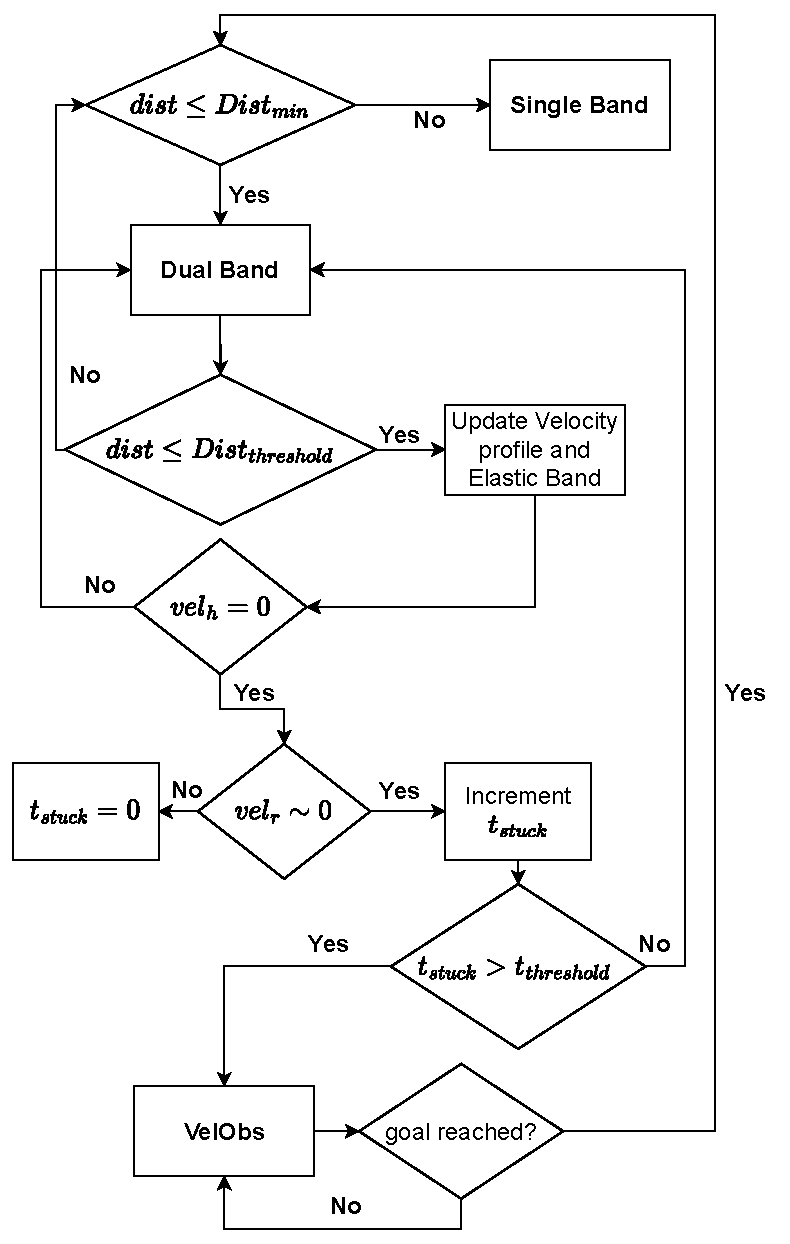
\includegraphics[width=0.78\columnwidth]{images/chapter3/final_flow_chart.pdf}
\caption{Mode transition procedure. \textit{dist} is the current distance between the closest human and the robot, $Dist_{min}$ is the minimum value of \textit{dist} to add a double band and $Dist_{threshold}$ is the minimum cutoff \textit{dist} to initiate transition between \textbf{Dual Band} and \textbf{VelObs}. $vel_h$, $vel_r$ are the velocities of the human and the robot. $t_{stuck}$ is the amount of time the robot's velocity is nearly zero, and $t_{threshold}$ is the time to wait before triggering the transition to \textbf{VelObs} mode. Note that, under $Dist_{threshold}$, the elastic band and velocity profile are changed irrespective of the mode of planning. The transition loop resets after reaching the navigation goal.}
\label{mode_shift}
\end{figure}

Now we move on to the explanation of the decision-making process involved in transitioning between the above modalities. Since HATEB-2 has three modes of planning, it has the following two mode transitions: 
\begin{enumerate}
    \item \textbf{Single Band} $\leftrightarrow$ \textbf{Dual Band}\footnote{$\leftrightarrow$ represents two side transition}
    \item \textbf{Dual Band} $\rightarrow$ \textbf{VelObs}.
\end{enumerate}

The transition procedure and decision-making loop are presented in Fig. \ref{mode_shift}. The decision concerning the transition from \textbf{Single Band} to \textbf{Dual Band} is dependent on a cutoff distance, $Dist_{min}$. $Dist_{min}$ is the distance between human and robot, above which the influence of humans on the robot's trajectory is negligible. If the current distance of the robot from any human is less than $Dist_{min}$, the planning shifts from \textbf{Single Band} to \textbf{Dual Band} and vice versa. Therefore it is a double-sided transition, and it is indicated by `$\leftrightarrow$'. $Dist_{min}$ can be chosen based on several factors and the present environment of the robot. During the development of this thesis, we have taken a distance of \SI{10}{\metre} for $Dist_{min}$.

From Fig. \ref{mode_shift}, we can see that the second transition only occurs when humans and the robot are under a specified distance, called the $Dist_{threshold}$. Under this $Dist_{threshold}$, the robot's maximum velocity is reduced, and the homotopy class change is constrained to make the robot's motion more legible for humans. The weight of the proxemics constraint is also reduced under this distance to allow the planner to find a solution in near proximity to humans. $Dist_{threshold}$ is taken as $2.5m$ for the most part of this work. This mode of \textbf{Dual Band} with all these changes is the intermediate mode we mentioned previously. Under this intermediary mode, the transition from \textbf{Dual Band} to \textbf{VelObs} mode occurs when the following situation is detected:

``\textit{The human under co-navigation with the robot stops proceeding towards the predicted goal, and the robot either stops or oscillates near this human for more than a specified amount of time without any progress towards the goal}''.

The amount of time chosen is arbitrary and can be tuned depending on the context. As it can be seen from the transition loop, the above condition is tested using the human's velocity ($vel_h$), the robot's velocity ($vel_r$) and a time threshold ($t_{threshold}$). For all the experiments presented in this thesis, the waiting time to trigger this shift is taken as \SI{2}{\second}, i.e., $t_{threshold} = \SI{2}{\second}$. Therefore, the robot does not stay frozen for long and quickly resolves the `\textit{entanglement problem}'. The transition from \textbf{Dual Band} to \textbf{VelObs} is one-sided, indicated by `$\rightarrow$' and does not happen the other way around. As this transition occurs mostly at the human-robot crossing, it is intuitive to assume that the human would be behind the robot and no longer interferes with the robot's trajectory after the transition. This assumption also reduces the cost of computation as we no longer plan for stationary humans. The mode transition loop resets once the robot reaches a navigation goal. If the goal change occurs in between, the robot continues to stay in the same mode as before the change, and the transitions may (\textbf{Single} or \textbf{Dual}) or may not (\textbf{VelObs}) occur. 

An important point to emphasise here is that all the situation analysis and mode shifting happens within the local trajectory planning during the robot's navigation to a specified goal. Therefore, HATEB-2 inherits all the advantages of proactive trajectory planning while reducing its limitations. This method of planning is different from the ones proposed by \cite{qian2013decision} or \cite{mehta2016autonomous}, where there is a higher level of decision-making that chooses between different possible navigation modes (or actions). Our system shifts between planning modes rather than navigation modes. HATEB-2 also incorporates some changes and modifications to the previous version of \acrshort{hateb} to improve legibility, and we present these in the next section.

 
\section{Improving the Legibility in HATEB-2}\label{improve_legible}
In addition to the situation assessment at the planning level, HATEB-2 proposes some new human-robot social constraints for HAN and modifies some modules in \acrshort{hateb}. All these proposals and modifications aim to increase the legibility of the robot's navigation and hence, can lead to an increase in acceptability. We present the new human-aware constraints (or human-robot social constraints) before moving on to the other modifications.

\subsection{New Human-Aware Constraints}
We propose two new human-aware constraints for HAN that increase the legibility of the robot's navigation. The first constraint is inspired by the work presented in \cite{kruse2014evaluating}. This constraint restricts the rapid velocity changes in the human vicinity as concluded by \cite{kruse2014evaluating}. The second one is an improved \textit{\acrfull{ttc}} constraint that was introduced by \acrshort{hateb}.

\subsubsection{Updated Robot Velocity Constraint}
In the place of a constant velocity, we assigned a non-linear profile for the velocity of the robot, which slows down the robot up to 75\% in the close vicinity of the human. This change reduces the rapid change in velocity around humans and leads to lesser confusion. The velocity function used in this constraint is given as follows:
\begin{equation}
    v(d) = min(1.0,max(10^{d-2},0.25))
    \label{vel_eq}
\end{equation}
where $d$ is the distance between the human and the robot and $v$ is the velocity of the robot. The above equation induces a rapid decrease in the maximum attainable velocity of the robot from \SI[per-mode=symbol]{1}{\metre\per\second} at $d=\SI{2}{\metre}$ to \SI[per-mode=symbol]{0.25}{\metre\per\second} at $d \leq \SI{1.4}{\metre}$ (personal zone in proxemics).

\subsubsection{TTCPlus Constraint}
Time-to-collision, as per its name, calculates the time the robot takes to collide with the human from the current position and velocity. 
\begin{figure}[!h]
\centering
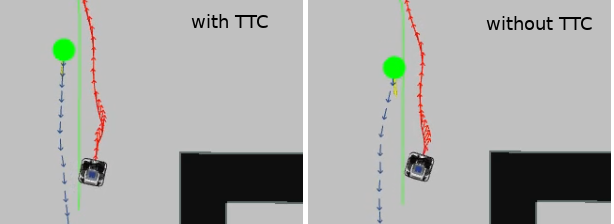
\includegraphics[width=0.9\columnwidth]{images/chapter3/ttc_importance_updated.png}
\caption{Intention show of the robot with and without \textit{\acrshort{ttc}}. Inclusion of \textit{TTC} or \textit{TTCplus} constraint results in an early intention show as can be seen from the picture on left. Even though the difference seems small from the pictures, this corresponds to more than half a meter in the real world. The robot's trajectory is shown in red, while the human's trajectory is shown in blue.}
\label{ttc_imp}
\end{figure}
The main advantage of including \textit{\acrshort{ttc}} constraint is better trajectory planning with early intention-show by making the robot move quickly towards the intended direction of its motion. This can be seen in Fig.  \ref{ttc_imp}. Although the difference seems small in the image, it is more than half a meter in the real world. The original implementation in~\cite{khambhaita2017viewing} computes the error at every time step and adds it to the optimization. This implementation results in many false negatives that affect the quality of the trajectory. To decrease the number of false alarms while maintaining the advantages of the constraint, we have to regulate the addition of the error to the optimization. The regulation is implemented in HATEB-2 as follows: 
\begin{equation}
error = 
     \begin{cases}
       ttc_{error}\ &\quad\text{if} \ t_a > t_d\ \text{and}\ t_m < \kappa t_d\\
       0,&\quad\text{otherwise}\\
     \end{cases}
     \label{ttc_eq}
\end{equation}
where $t_d$ is the threshold time, $t_a$ is the cumulative time with positive $ttc_{error}$ and $t_m$ is the cumulative time with zero $ttc_{error}$. $t_a$ is reset whenever $t_m \ge \kappa t_d$ and $t_m$ is reset when a positive error is observed. $\kappa$ is 
a constant determining how often the $ttc_{error}$ is added to the optimization, and in this work, we take $\kappa = 5$ based on empirical analysis. This new implementation shown in Eq.~\eqref{ttc_eq}, called \textit{TTCplus}, decreases the number of false negatives, avoiding unnecessary oscillations and improving the quality of trajectory. Hence, \textit{TTCplus} eliminates the drawbacks of \textit{\acrshort{ttc}} while preserving its properties of early intention-show.

\subsection{Modified Elastic Band}
\begin{figure}[!h]
\centering
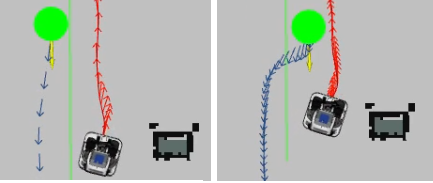
\includegraphics[width=0.9\columnwidth]{images/chapter3/tight_band_new.png}
\caption{Modified Elastic band. The blue trajectory is of the human, and the red one is of the robot. Tightening of the elastic band results in very close pose predictions in the trajectories and slower velocities. The picture on the left shows the trajectories before band tightening, and the one on the right shows the latter.}
\label{band_tight}
\end{figure}
The default settings of the elastic band allow it to rapidly change the homotopy\footnote{In mathematics, two paths are homotopic if their endpoints are fixed, and one path can be continuously deformed into another within a specified region.} class. This change is good when the robot is at a large distance from humans. At closer distances, it may lead to the loss of legibility, as the study in \cite{kruse2014evaluating} says. Hence, we address this issue by restricting the changing of the homotopy class under the threshold distance, \textit{DistThreshold}. This restriction is implemented by decreasing the time interval between consecutive poses, which tightens the elastic band and decreases the possibility of homotopy class change, as shown in Fig. \ref{band_tight}. This figure shows the snapshots of the trajectories before and after the online band tightness modification. The picture on the right side clearly shows a significant increase in the trajectory resolution, and hence, results in smoother path transitions.

\subsection{Better Human Predictions}
The better the estimates of humans, the better the proactive planning can plan the joint trajectories. Therefore, we have made the following improvements in HATEB-2 to have better estimates and path predictions for humans.

\subsubsection{Human Velocity Estimate}
The nominal velocity of a human was assumed to be constant in the previous work. However, this assumption leads to a trajectory plan that does not necessarily comply with the current human trajectory. Although HATEB-2 being a proactive planner, quickly re-plans and adapts, this wrong estimate can sometimes lead to unexpected behaviours of the robot. Therefore, a moving average filter-based estimation of velocity is added to the human prediction to avoid this and provide an adaptive velocity estimate for optimization.

\subsubsection{Human Goal Prediction}
In \acrshort{hateb}, human goals were assumed to be behind the robot for path prediction. However, this is not necessarily true in many cases, and the human destination might even change during the navigation. Therefore, we try to include better human goal predictions into the system and address the changes in the human goal during the planning process. If we know a set of possible destinations for humans in an environment, we can predefine a set of goal positions for humans. Ferrer et al.~\cite{ferrer2014bayesian} proposed a methodology to estimate the possible goal among these predefined goals based on the history of motion of the human. HATEB-2 adopts this goal estimation framework to improve human estimations. It quickly adapts to the changes in the human goal and re-plans, as shown in Fig. \ref{goal_predict}, making it more adaptable to real-world scenarios.
\begin{figure}[!h]
\centering
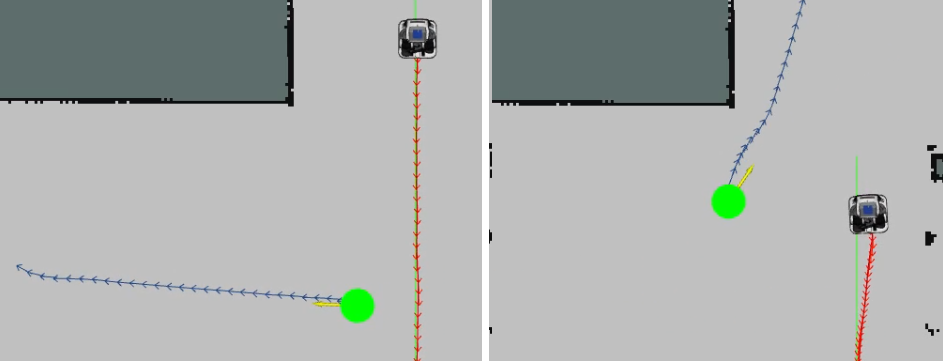
\includegraphics[width=0.9\columnwidth]{images/chapter3/goal_predict_updated.png}
\caption{Human goal prediction in HATEB-2. On the left side, the initial predicted goal, and the calculated trajectory by HATEB-2 are shown. On the right, human decides to move in a different direction, and HATEB-2 predicts a new possible goal and calculates path. The robot's trajectory is shown in red, while the human's trajectory is shown in blue.}
\label{goal_predict}
\end{figure}

\section{Results in Simulation}\label{results_chap3}
Various experiments are conducted using PR2\footnote{\url{http://wiki.ros.org/Robots/PR2}} robot and the simulated humans in MORSE~\cite{echeverria2011modular} to demonstrate the capabilities of HATEB-2. Two different environments are used to simulate different human-robot navigation scenarios. Both \textit{Qualitative} and \textit{Quantitative} analysis is performed, and the results are presented. The first three experiments presented in this section show the \textit{Qualitative} analysis, highlighting the improvements in HATEB-2 and the roles of situation assessment and proactive planning in HAN. In all three experiments, the human agent is manually controlled using a Joystick.

%%%%%%%%%%%%%Need to find a way %%%%%%%%%%%%%
% \footnote{Source code for this version of HAN system is available at \url{https://github.com/sphanit/hateb_local_planner/tree/hateb_new}}
%%%%%%%%%%%%%Need to find a way %%%%%%%%%%%%%

\subsection{Entanglement Resolution through Mode Shifting}
One of the main drawbacks of \acrshort{hateb} is the \textit{entanglement} issue presented previously. With the introduction of decision-making and mode transitioning in HATEB-2, this \textit{entanglement problem} is resolved, and the robot finally reaches the goal without getting stuck.  The various stages of this \textit{entanglement} resolution are illustrated in Fig. \ref{resolve}.  When the human stops moving and blocks the robot, a new trajectory is planned, and the transition from \textbf{Dual Band} mode to \textbf{VelObs} mode occurs (Fig. \ref{resolve} (a, b)). Since the human's velocity is zero, the \textbf{VelObs} mode does not plan any trajectory for the human until he starts moving again. During this time, the robot escapes from the \textit{entanglement} and starts following its trajectory to the goal, as seen in Fig. \ref{resolve} (c) and (d).   
\begin{figure}[!h]
\centering
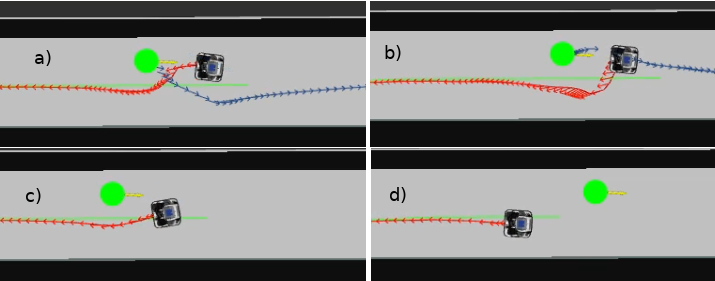
\includegraphics[width=0.9\columnwidth]{images/chapter3/mode_change.png}
\caption{HATEB-2 solving the \textit{entanglement}. The various stages of \textit{entanglement} resolution are as shown: a) Detection of Entanglement: The \textit{entanglement} is detected based on the human velocity and the current distance between human and robot. b) Re-planning: HATEB-2 tries to re-plan the trajectory before changing the mode c) Mode Transition: Mode transition occurs as the human is still and no longer moves. d) Execution of new plan: Finally, the robot executes the planned trajectory reaching the expected goal. The robot's trajectory is shown in red, while the human's trajectory is shown in blue.}
\label{resolve}
\end{figure}

\subsection{Advantages of Proactive Planning}
We present two experiments to show the advantages of proactive planning in HAN. The second experiment tests proactive planning and situation analysis in a complex setting. It shows how HATEB-2 solves the navigation problem in a more legible way.

\subsubsection{Single Band vs Double Band}
The single band refers to the addition of an elastic band only to the robot along with the human-aware constraints, whereas the double band (or dual band) includes the addition of an elastic band to the human as well. We test the following hypothesis to see if the double band has any advantage over the single band: 

\textit{``The  presence of an elastic band for human and co-planning allows the robot to predict the human motion better and adapt its trajectory accordingly.''}

\begin{figure}[!h]
\centering
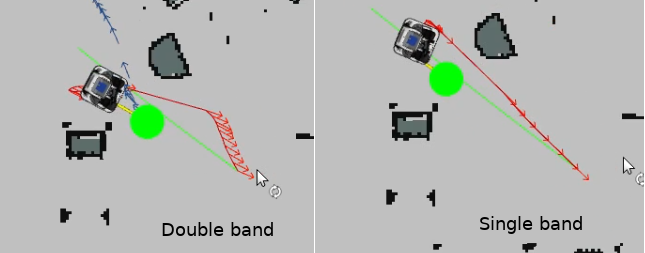
\includegraphics[width=0.9\columnwidth]{images/chapter3/door_tj.png}
\caption{Double band and single band trajectories while passing through a narrow passage. As the red trajectory corresponds to the robot, it can be observed from the picture on the left that double band based planning makes the robot back off proactively and provide a way for the human. Whereas single band based planning shown on the right reacts slowly and moves sideways to clear the way for the human.}
\label{door_tj_fig}
\end{figure}

To test the hypothesis, we controlled the human manually, tried to block the robot's trajectory, and observed the reactivity of the robot. We conducted two different experiments (in open space and narrow passage (Fig. \ref{hateb2})), and in both experiments, the robot reacted slowly while using a single band. However, while using the double band, the robot proactively backs off as the human moves towards it. Therefore, we can say that our hypothesis is correct,  and the inclusion of an elastic band for humans is advantageous for HAN planning. These experiments can be seen clearly in the video\footnote{\url{https://youtu.be/xEG4e-Y9z8g}\label{vd_ln}}. Snapshots of this experiment in case of the narrow passage scenario are shown in Fig.~\ref{door_tj_fig}


\subsubsection{Pass through Narrow Opening}
This experiment can be thought of as passing through a door where only a single person can fit. Suppose two persons arrive at the narrow opening at the same time, one of them has to back off and give way for the other to pass through. We tried to simulate this scenario\textsuperscript{\ref{vd_ln}} in the human-robot co-navigation, and we want the robot to back off and give way to the human. To increase the complexity of this problem further, human crosses the opening and stops close to this opening. Enough space is present for the robot to pass through, but the trajectory might need re-planning. This scenario is shown in Fig. \ref{hateb2}. 
\begin{figure*}[!h]
\centering
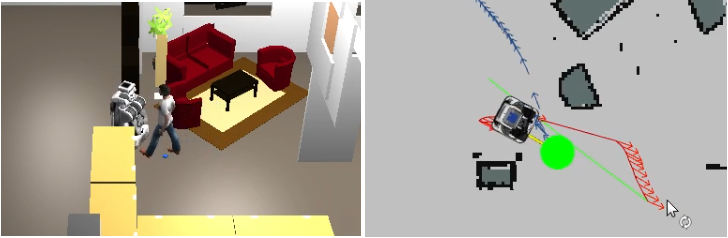
\includegraphics[width=0.9\columnwidth]{images/chapter3/hateb2.png}
\caption{Narrow passage passing scenario. In this scenario, the human and robot arrive at the common passage at the same time, and one should back off to provide a way for another. Otherwise, there exists no solution. This is one of the intricate situations addressed in this work, and the picture on the left shows the simulation of this scenario in MORSE. The right side picture shows the trajectories for the human (blue) and the robot (red), generated using the proposed framework, HATEB-2. It can be seen from the picture that the robot's trajectory (red) is making the robot move backwards and hence providing a way for the human.}
\label{hateb2}
\end{figure*}

% \begin{figure}[h]
% \centering
% 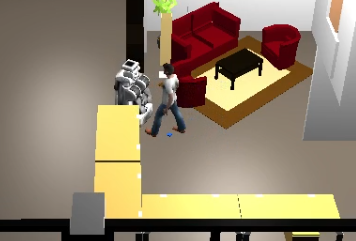
\includegraphics[scale=0.55]{./Images/door.png}
% \caption{Simulated narrow pass scenario in MORSE}
% \label{door_fig}
% \end{figure}

We have tested all three planners (\acrshort{hateb}, HATEB-2 and Single Band) in this scenario and snapshots of the trajectories at this crossing are shown in Fig. \ref{door_tj_fig} for both double band (\acrshort{hateb}, HATEB-2) and single band planning. Both \acrshort{hateb} and HATEB-2 reacted, in the same way, to back off and provide a way for the human, which is shown in the left picture of Fig. \ref{door_tj_fig}. Although they reacted similarly at this instant, \acrshort{hateb} gets stuck in \textit{entanglement} when the human stops moving after crossing the opening. HATEB-2 breaks this \textit{entanglement} and re-plans to reach the given goal. Coming to the case of the single band, the human has to stop in front of the robot and wait for the robot to back off and re-plan. The single band also solves this case as it does not suffer from \textit{entanglement} but with lesser reactive speeds. Also, note that the robot backs off in a double band scenario, whereas it tries to move aside in the single band case. 

\subsection{The Effect of New Human-Aware Constraints}
\textit{\acrshort{ttc}} constraint in \acrshort{hateb} makes the robot very reactive and leads to unnecessary oscillations, as mentioned previously. Fig. \ref{ttc_fig} shows the trajectory of the robot in the same scenario using \textit{\acrshort{ttc}} and \textit{TTCplus} constraints respectively.
\begin{figure}[h]
\centering
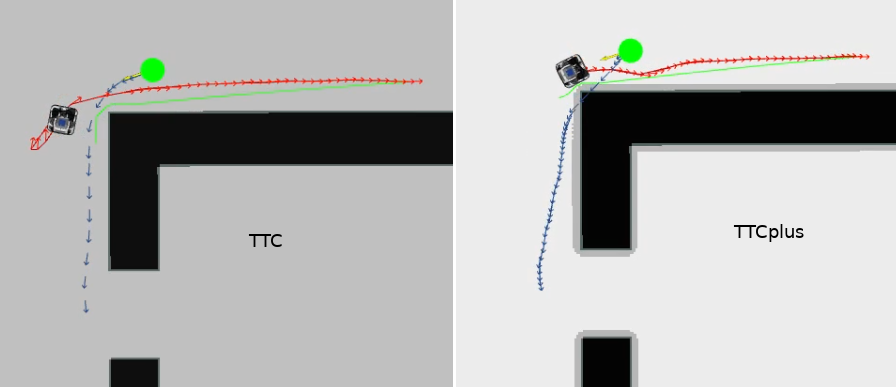
\includegraphics[width=0.8\columnwidth]{images/chapter3/ttc.png}
\caption{The original \textit{TTC} constraint-based trajectory shown on the left results in unnecessary oscillations due to exaggerated constraint. However, \textit{TTCplus} constraint regulates this exaggeration and results in a smooth trajectory as shown on the right. Note that the trajectory on the left is making the robot move backwards even when there is no necessity. The robot's trajectory is shown in red, while the human's trajectory is shown in blue.}
\label{ttc_fig}
\end{figure}
As we can see from the trajectory on the left, the plan using \textit{\acrshort{ttc}} constraint makes the robot back off further when it is already at a sufficient distance from the human. This exaggerated reaction results in long execution times apart from the oscillations. The trajectory planned using \textit{TTCplus} in HATEB-2 is shown on the right, and it can be clearly seen from Fig. \ref{ttc_fig} that this trajectory results in faster execution as it removes the problem of oscillations. The change in the elastic band tightness can be seen in the right part of Fig. \ref{ttc_fig}. This change, coupled with the reduced velocity in the close vicinity of the human, helps the human choose the path without confusion. Clear differences in the trajectory followed, and the effect of all these constraints can be seen in the video\footnote{\url{https://youtu.be/xEG4e-Y9z8g}}. 

\subsection{Quantitative Comparison between HATEB and HATEB-2}
To perform the \textit{Quantitative} analysis, five different experiments were conducted, and each experiment was repeated 10 times using \acrshort{hateb} and HATEB-2. The list of the experiments performed is given in Table~\ref{results}. The experiment \textit{`Narrow opening 1'} is same scenario presented in Fig.~\ref{hateb2}, whereas \textit{`Narrow opening 2'} corresponds to similar case with opening that can be seen in Fig. \ref{ttc_fig}. \textit{`L-crossing'} is the same experiment that is shown in Fig. \ref{ttc_fig} and finally \textit{`Narrow corridor'} and \textit{`Wide space'} represents the scenarios presented in Fig. \ref{stuck}. 

In all these experiments, the goal of the human was assumed to be behind the robot, and the human executed the trajectory planned by the corresponding local planner. A set of five metrics are used to analyse the results: 1) Initial plan length, $ipl$, 2) Total time for completion, $ct$, 3) Traversed path length, $tpl$ 4) Minimum distance from human, $d_{min}$ and 5) Length deviation factor, $\alpha$. The minimum distance from the human metric, $d_{min}$, refers to the closest distance between the human and the robot while executing a planned trajectory. The length deviation factor, $\alpha$, is defined as follows:
\begin{equation}
    \alpha = \frac{|tpl - ipl|}{ipl}
    \label{alp}
\end{equation}
where $|\ \ |$ denotes the absolute value. After determining $ipl$ and $tpl$ from the experiments, $\alpha$ is calculated using Eq. \eqref{alp}.
\begin{table*}[ht!]
    \centering
    \begin{tabular}{|c|c|c|c|c|c|}
    \hline
     & \multicolumn{5}{c|}{HATEB} \\
    \cline{2-6}
    Experiment & $ipl (m)$ & $tpl (m)$ & $ct (s)$ & $d_{min} (m)$ & $\alpha$ \\
    % & $ipl(m)$ & $tpl(m)$ & $ct(s)$ & $d_{min}$(m) & $\alpha$\\
    \hline
    \textit{Narrow opening 1} & \bf{5.26} & \bf{5.94} & \bf{13.63} & \bf{0.72} & \bf{0.13} \\ 
    % & 5.3597 & 6.3423 & 17.6350 & 0.539 & 0.1903\\
    \hline
    \textit{Narrow opening 2} & 8.71 & 11.09 & 24.29 & 0.14 & 0.27 \\
    % & \bf{9.0233} & \bf{9.1606} & \bf{21.9319} & \bf{0.1505} &\bf{0.0152}\\
    \hline
    \textit{L-crossing} & 10.66 & 15.29 & 32.56 & 0.14 & 0.43 \\
    % & \bf{13.4602} & \bf{13.0613} & \bf{29.8967} & \bf{0.3430} &\bf{0.0296}\\
    \hline
    \textit{Narrow corridor} & 8.51 & \bf{13.18} & \bf{27.92} & \bf{0.72} & 0.55 \\
    % & \bf{12.8807} & 13.2372 & 30.8850 & 0.4845 &\bf{0.0277}\\
    \hline
    \textit{Wide space} & 8.51 & \bf{9.54} & \bf{19.81} & 0.72 & 0.12 \\
    % & \bf{9.8575} & 9.6781 & 22.2517 & \bf{0.8274} &\bf{0.0182}\\
    \hline
    & \multicolumn{5}{c|}{HATEB-2}\\
     \cline{2-6}
    \hline
    \textit{Narrow opening 1} & 5.36 & 6.34 & 17.63 & 0.54 & 0.19\\
    \hline
    \textit{Narrow opening 2} & \bf{9.02} & \bf{9.16} & \bf{21.93} & \bf{0.15} &\bf{0.02}\\
    \hline
    \textit{L-crossing} & \bf{13.46} & \bf{13.06} & \bf{29.90} & \bf{0.34} &\bf{0.03}\\
    \hline
    \textit{Narrow corridor} & \bf{12.88} & 13.24 & 30.88 & 0.48 &\bf{0.03}\\
    \hline
    \textit{Wide space} & \bf{9.86} & 9.68 & 22.25 & \bf{0.83} &\bf{0.02}\\
     \hline
    \end{tabular}
    \caption{Mean values of the metrics over 10 repetitions. $ipl$: Initial path length, $tpl$: Traversed path length, $ct$: Completion Time of the experiment, $d_{min}$: Minimum distance between human and robot during the execution of the trajectory in the given experiment. $\alpha$: Length deviation factor.}
    \label{results}
\end{table*}

All these metrics are calculated for each experiment, and the mean value over 10 experiments is presented in Table~\ref{results}. The values highlighted in bold correspond to the best values in the given experiment. The evaluation of the best values for the metrics is done in the following manner. For $ipl$, the value closest to the $tpl$ is taken as the best value, as it suggests that the initial plan is very close to the traversed path. In case of $tpl$ and $ct$, smaller value represents the best value. The greater the distance of the robot from the human, the more the safety factor for the human, and hence, the larger distance is the best value. Finally, the lower value of $\alpha$ represents the lesser deviation from the initial plan and hence shows better performance of the planner. By observing the values of $\alpha$ from the table, it can be inferred that HATEB-2 performs better than \acrshort{hateb} in all the cases, except \textit{`Narrow opening 1'}. In all these scenarios, it can also be seen that $ipl$ differs less from $tpl$, and hence, we can say that HATEB-2 predicts a better plan than \acrshort{hateb}. The cause of this result can be directly associated with the improvements in human prediction and the new $TTCplus$ constraint, thereby demonstrating the importance of human prediction in HAN. As the maximum allowed velocity decreases below $Dist_{threshold}$ in HATEB-2, an increase in $ct$ is expected, and it is true in 3 out of the 5 cases. In \textit{`Narrow opening 2'} and  \textit{`L-crossing'} cases, HATEB-2 has lesser $ct$ than \acrshort{hateb} and this is because of the improved \textit{\acrshort{ttc}} constraint, \textit{TTCplus}. Since \acrshort{hateb} uses the original \textit{\acrshort{ttc}}, the robot suffers from unnecessary oscillations and results in a longer path length, $tpl$ as well as $ct$. It can be observed that HATEB-2 completely outperforms \acrshort{hateb} in these two scenarios. Although \acrshort{hateb} has better $tpl$ values in the other three scenarios, the $tpl$ values of HATEB-2 are very close to those of \acrshort{hateb}. Finally, it can be said that the overall performance of HATEB-2 is better than \acrshort{hateb}.

\section{Real-World Tests}\label{real_chap3}
In this section, we present the experiments we have conducted using the proposed framework. We have ported the framework to Pepper\footnote{\url{https://www.ald.softbankrobotics.com/en/pepper}} robot and used it for this study. Since the main objective is to study the navigation framework, we used the OptiTrack\footnote{\url{http://www.optitrack.com/}} motion-capturing system to track humans. The localization of the robot in the map is done using the localization technique based on ArUco\footnote{\url{https://chev.me/arucogen/}} markers.
\begin{figure}[!h]
\centering
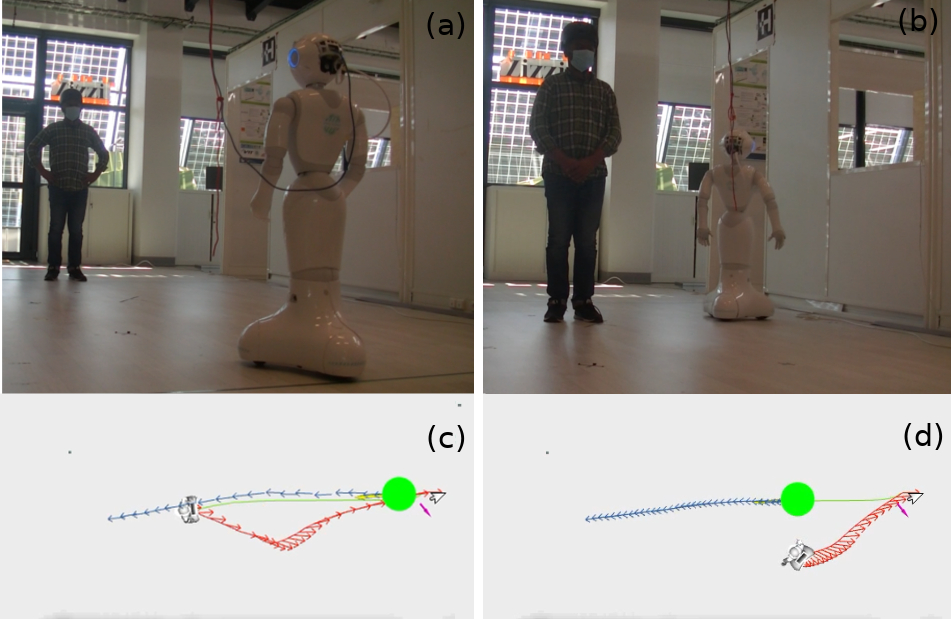
\includegraphics[width=0.9\columnwidth]{images/chapter3/pepper_case_1_new}
\caption{Human follows his path without disturbing the robot. (a) Initial positions (b) Intermediate positions. (c) and (d) are the trajectories at (a) and (b) respectively. In (d), the band tightening can be seen as the robot is close to the human. Red: The robot's trajectory is shown in red, while the human's trajectory is shown in blue.}
\label{case1_pepper}
\end{figure}

\begin{figure}[!h]
\centering
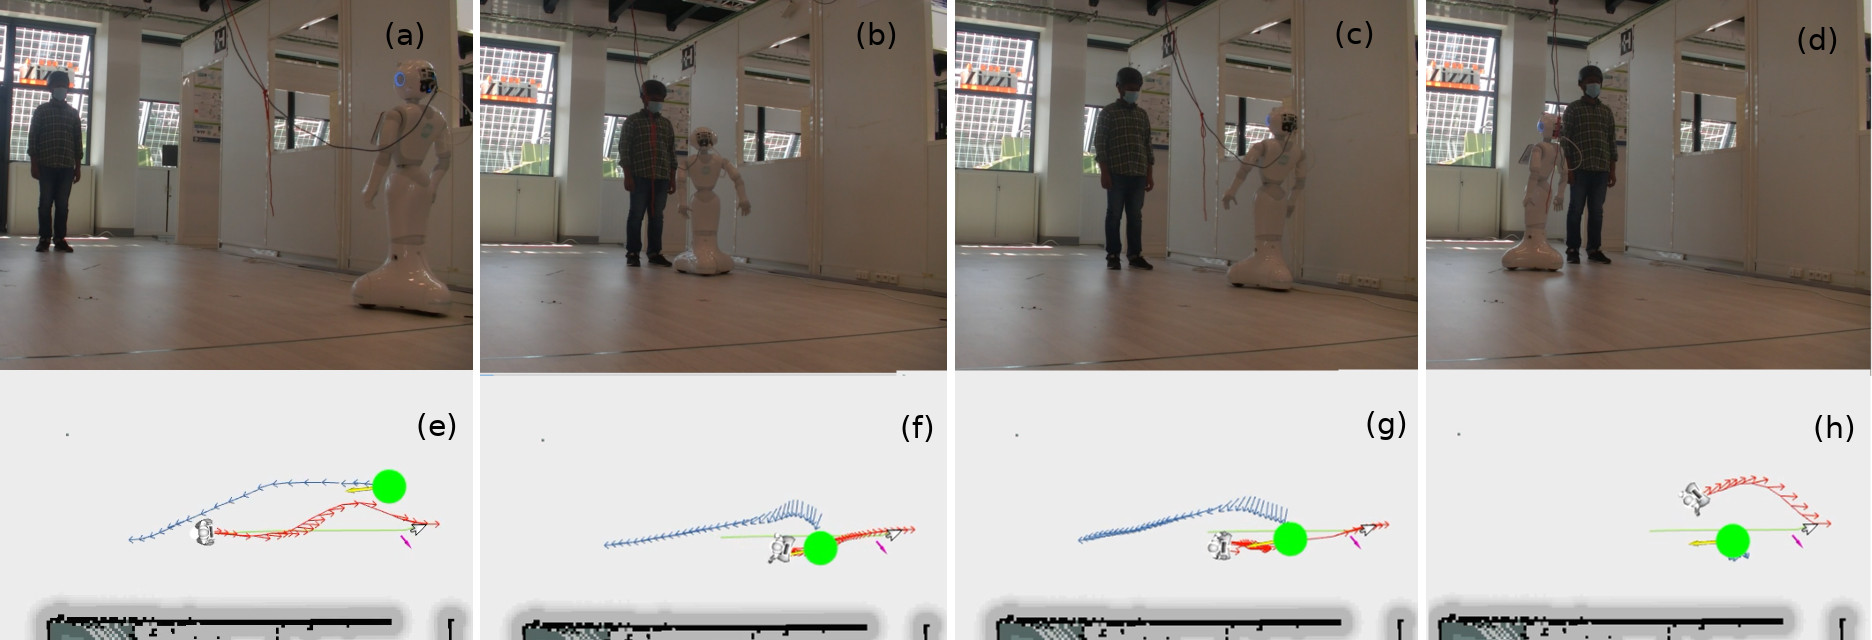
\includegraphics[width=0.9\columnwidth]{images/chapter3/pepper_case_2}
\caption{Entanglement resolution in a real-world scenario. Here the human goes out of his path and blocks the robot's planned path (f). While trying to block the path, he moves very close to the robot, as can be seen from (f). Therefore, the robot backs off (g) before resolving the entanglement and finding an alternative path (h). (a)-(d) represent different positions of the robot during the experiment, and (e)-(h) show the planned trajectories at these positions. The robot's trajectory is shown in red, while the human's trajectory is shown in blue.}
\label{case2_pepper}
\end{figure}

We have conducted two experiments to check the capabilities and improvements in HATEB-2. In the first experiment, shown in Fig.~\ref{case1_pepper}, the human moves along his path without blocking the way for the robot. It can be seen from Fig. \ref{case1_pepper} that the robot continues to navigate on the same side and follow a path similar to the initially planned path. We can also observe the band tightening in Fig. \ref{case1_pepper} (d) as the human is close to the robot. In the second experiment, the human goes out of his path and blocks the robot's planned path. Two kinds of scenarios are possible depending on how the human acts in this setup. If the human goes very close to the robot, the robot has to back up before resolving the \textit{entanglement problem}. In the other case, where the human is at a nominal distance from the robot, only \textit{entanglement} resolution happens. These two cases are presented in the video. However, we have presented only the first scenario in this section as it brings out more capabilities of the system. This is shown in Fig. \ref{case2_pepper}. In Fig. \ref{case2_pepper} (f), human goes very close to the robot and hence the robot backs off (Fig. \ref{case2_pepper} (g)) before resolving the \textit{entanglement}. Finally, the \textit{entanglement} is resolved (Fig. \ref{case2_pepper} (h)) and the robot proceeds to its goal.

\section{Conclusion}\label{conclude_chap3}
In this chapter, we have proposed a new framework combining proactive planning and decision-making to handle human-robot co-navigation, called HATEB-2. This framework includes three different modes of planning, namely, \textbf{Single Band}, \textbf{Dual Band} and \textbf{VelObs}. Switching between these modes allows for solving many complex human-robot cooperative navigation problems. We have presented details of these different modes of planning and also talked about the modifications made in \acrshort{hateb} before including it in HATEB-2. These modifications remove some of the drawbacks of \acrshort{hateb} apart from the improvements. We have also presented the improvements made in human prediction and estimation. We performed several experiments in various intricate situations and then provided a detailed analysis of the results. Results show that HATEB-2 have an overall better performance. The framework was finally tested on a real robot platform, and the results were presented.

It is evident that HATEB-2 can handle intricate human-robot navigation scenarios better when compared to \acrshort{hateb}. However, it still carries some of the limitations of \acrshort{hateb}. One of the main drawbacks is the computational complexity with a growing hypergraph as more humans are added to the planning. Even though humans' predictions were improved in HATEB-2, path planning still needs improvements. In the next chapter, we discuss how these limitations were handled to scale our planning system to tens of humans. One of the limitations of the \textit{\acrshort{ttc}} constraint is that it works well when the robot and human are approximately on the same line of travel or with very small parallel gaps. If the line of travel has a large parallel gap, it is not very effective. The same limitations apply to \textit{TTCplus} as well. Therefore, we introduce new social constraints to address these limitations and effectively handle parallel travel.          
